\documentclass[a4paper,twoside]{report}
%Rahmendatei f�r das Cover

\usepackage{graphicx}

\usepackage{epsf,amsthm,amsmath}
\usepackage[ngerman]{babel}
\usepackage[latin1]{inputenc}
\usepackage{graphicx}
\setlength{\parskip}{5pt plus 8pt minus 2pt}
\pagestyle{headings}

%----------------------------------------------------------------------
%  Makros
%----------------------------------------------------------------------
%\usepackage{dsfont}
%\def\C{\mathds{C}}
%\def\F{\mathds{F}}
%\def\R{\mathds{R}}
%\def\N{\mathds{N}}
%\def\Z{\mathds{Z}}
%
%\newcommand{\bra}[1]{\langle#1|}
%\newcommand{\ket}[1]{|#1\rangle}
%\newcommand{\braket}[2]{\langle#1|#2\rangle}
%\newcommand{\ketbra}[2]{|#1\rangle\langle#2|}
%\newcommand{\projektor}[1]{|#1\rangle\langle#1|}
%\newcommand{\schnitt}[2]{
%   \raise3pt\vbox{\moveright6.5pt\hbox{$#1$}}\hspace*{-4pt}\Bigm/
%   \lower3pt\vbox{\moveleft6.5pt\hbox{$#2$}}}
%
%\newcommand{\includeeps}[2]{
%   \def\epsfsize##1##2{#2##1}
%   \centerline{\epsffile{#1}}}
%
%\newtheorem{satz}{Satz}[chapter]
%\newtheorem{bem}[satz]{Bemerkung}
%\newtheorem{lem}[satz]{Lemma}
%\newtheorem{defi}[satz]{Definition}
%\newtheorem{beispiel}[satz]{Beispiel}
%----------------------------------------------------------------------

\begin{document}
\begin{titlepage}
\ \vfill
\Large
\begin{center}
{\LARGE\bf Proseminar} \\[1cm]
{\huge\bf K"unstliche Intelligenz\par}
\vspace*{1cm}
\input unilogo
\unilogo{30}\\[1cm]
{\bf Universit"at Karlsruhe (TH)}\\
{Fakult"at f"ur Informatik}\\
{\em Institut f"ur Algorithmen und Kognitive Systeme}
\vfill
Prof.~Dr.~J.~Calmet\\
Dipl.-Inform.~A.~Daemi
\vfill\vfill 
Wintersemester 2003/2004
\vfill
\vfill
\end{center}
\end{titlepage} 
% 
%\newpage
%\thispagestyle{empty}
%\ 
%\newpage 
\thispagestyle{empty}
\ 
\vfill
\noindent
Copyright $\copyright$ 2003\\
Institut f"ur Algorithmen und Kognitive Systeme\\
Fakult"at f"ur Informatik\\
Universit"at Karlsruhe\\
Am Fasanengarten 5\\
76\,128 Karlsruhe

%\newpage 
%\thispagestyle{empty}
%\ 
%\newpage 



\title{Allgemeine und Heuristische Suchverfahren}
%Namen der Autoren (�NDERN!!)
\author{Henning \\ Clemens Lode}

%Rahmendatei f�r Titel, Autor und Inhaltsverzeichniss
\date{}
\maketitle

%\thispagestyle{empty}
%\newpage 

\pagenumbering{roman}
\tableofcontents

%\newpage 
\pagenumbering{arabic}


\setcounter{chapter}{0}
\chapter{Allgemeine und Heuristische Suchverfahren}

%---------------------------------------------------------
%Hier beginnt das eigentliche Dokument 
%---------------------------------------------------------
%Die Ausarbeitung sollte immer eine Einf�hrung in die behandelnden Themen enthalten
\section{Einleitung}

Neben der Suche nach ueberhaupt einer Loesung, geht es in diesem Vortrag vor allem um das Suchen nach einer moeglichst optimalen oder gar der optimalen Loesung. Die meisten Probleme sind komplexer Natur und somit nicht eindimensional, also muessen wir zuerst eine Abbildung der jeweiligen Loesung auf N oder R finden um entscheiden zu koennen, welche der betrachteten Loesungen besser als eine andere ist.

\section{Allgemeine Suchverfahren}


\section{Heuristische Suchverfahren}

\subsection{Unterschiede zu allgemeinen Suchverfahren}

Informierte Suchverfahren basieren auf Heuristiken, besitzen also manuell einprogrammiertes problemspezifisches Wissen.
Dabei handelt es sich um Algorithmen die in vielen Faellen eine bessere durchschnittliche Suchdauer besitzen als Algorithmen uninformierter Suchverfahren, waehrend sie, zumindest die vollstaendigen Algorithmen, ebenfalls den schlechtesten Zeitaufwand von O(\(b^{m}\)) besitzen.
%Anschaulich gesprochen weisen die Heuristiken den Algorithmen einen Weg durch den Suchraum, der wahrscheinlich schneller zum Ziel fuehrt als bei konventioneller Herangehensweise.

\subsection{Gruppen von heuristischen Suchverfahren}
Man kann die Algorithmen in 2 Gruppen einteilen. Vertreter der ersten Gruppe setzen sich Schritt fuer Schritt die Loesung zusammen, Vertreter der zweiten Gruppe betrachten fertige, nicht unbedingt optimale, Loesungen und versuchen diese iterativ zu verbessern.
Die Grundidee bei beiden Gruppen ist, dass man jeweils alternative Schritte bzw. Loesungsmoeglichkeiten vergleicht und jeweils moeglichst die waehlt, die auch zu einer optimalen Loesung fuehren.
Dazu waehlt man eine nicht-negative Heuristikfunktion h, die einem Zustand n einen Wert zuweist. Je niedriger h(n), desto besser ist der Zustand n. h(n)=0 bedeutet, dass n die optimale Loesung darstellt.
Ausserdem benoetigen wir eine Auswahlfunktion i, die uns einen neuen Zustand, also ein Loesungsschritt der bzw. eine Loesungsmoeglichkeit die wenn moeglich noch nicht betrachtet wurde, zurueckgibt.
Das Problem zu jeder Aufgabenstellung ist also erst einmal das Finden einer Funktion h und i die das bewerkstelligen. Eine der Aufgabenstellung nicht angepasste Heuristik und Auswahlfunktion fuehren zu laengerer Laufzeit oder gar zu Sackgassen und Schleifen.

\subsection{Finden einer heuristischen Funktion} 
%~~

Um eine Funktion h zu finden, die den Suchvorgang moeglichst verkuerzt, bietet es sich an, ein sogenanntes "Relaxed Problem", also ein vereinfachtes Problem zu betrachten, bei dem bestimmte Beschraenkungen in der Loesungsschrittwahl aufgehoben sind. Damit erhalten wir eine moegliche Bewertung eines Loesungsschritt, wie weit wir von der optimalen Loesung entfernt sind.

Als Beispiel betrachten wir das sogenannte "8-puzzle" [2] Problem:

\begin{figure}
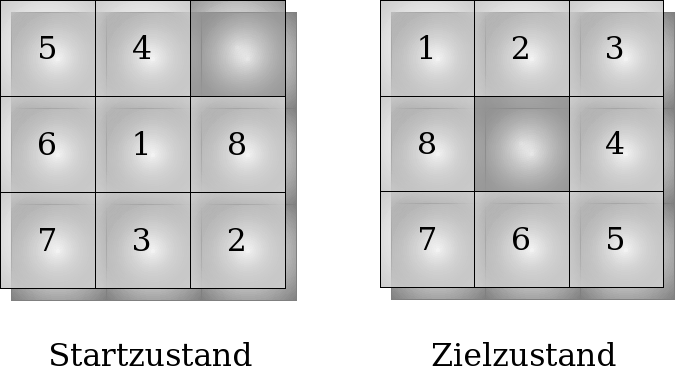
\includegraphics[scale=0.5]{8puz1.png}
\caption{Beispiel zum "8-Puzzle" Problem}
\end{figure}
                                                                                                                                                            

Beim "8-puzzle" Problem ist das Ziel, die Teile so zu bewegen, dass man vom Startzustand ausgehend den Zielzustand erreicht.
Die Beschraenkung ist hierbei, dass man immer nur 1 Teil bewegen darf und sich niemals 2 Teile auf einem Feld befinden duerfen.

%~~ ueberhaupt rein? :/
Da sich in jedem Schritt 2 (freies Feld in der Ecke), 3 (freies Feld am Rand) oder 4 (freies Feld in der Mitte) Teile bewegen duerfen, wuerde eine komplette Suche aller Moeglichkeiten mit Zugtiefe 20 zu 3.5*10\^9 oder, ignoriert man sich wiederholende Situationen, zu 9! Zustaende fuehren.[3]  ~~

Wie stellen wir nun fest, ob wir uns beim Bewegen eines Teiles auf die optimale Loesung zu bewegen oder uns entfernen?
Beim Ursprungsproblem koennen wir nur feststellen, ob ein Zustand dem Zielzustand entspricht oder nicht.
Wir muessen also ein vereinfachtes, sogenanntes "relaxed problem" ~~ finden, so dass Ueberschreitungen von Beschraenkungen nicht zu einem Ignorieren des Loesungsschritt bzw. der Loesung ~~ fuehrt.

Zuerst listen wir die Beschraenkungen noch einmal getrennt auf:

Ein Teil darf

1. pro Schritt nur 1 Feld und 

2. nicht schraeg und 

3. nur in ein freies Feld

verschoben werden

Heben wir in diesem Fall die Beschraenkung 3 einfach auf, duerfen sich also Teile auch auf besetze Felder bewegen, wissen wir, dass die Summe der Schritte der Teile von ihren aktuellen Positionen zu den Zielpositionen die minimale Zahl der Schritte ist, die wir zur optimalen Loesung benoetigen.
In diesem speziellen Fall wird das Manhattan distance genannt [4, Seite 102]
Hebt man zusaetzlich noch Beschraenkung 1 auf, erhaelt man eine Heuristik, die die Zahl der Teile die sich an falscher Position befinden beschreibt.

Nach [5, 102] ist die erste Heuristik der zweiten Heuristik mit weniger Beschraenkungen ueberlegen, fuehrt also zu einer Suche mit geringerer durchschnittlichen Suchdauer. ~~

Prueft man alle Kombinationen von Beschraenkungsaufhebungen erreicht man so eine fuer das jeweilige Problem optimale Loesung. Diesen Weg beschreitet ABSOLVER ~~ [6,103]
\\

\begin{figure}
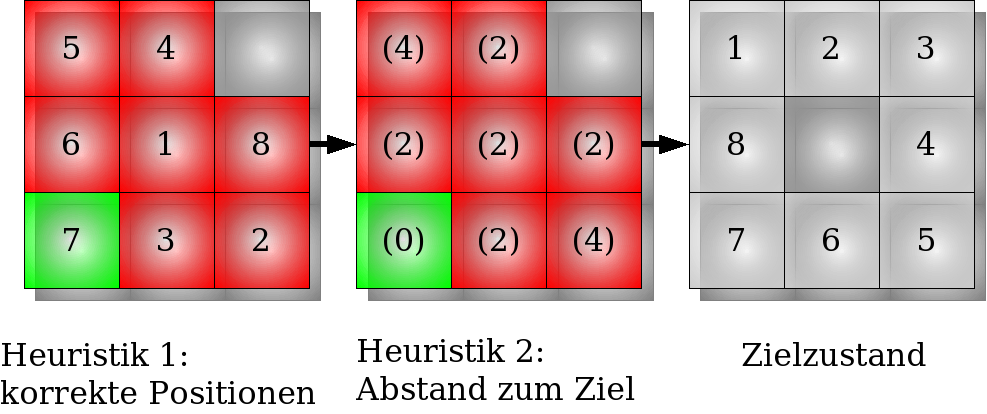
\includegraphics[scale=0.5]{8puz2.png}
\caption{2 moegliche Heuristiken zur Loesung von "8-puzzle"}
\end{figure}
                                                                                                                                                            
% text?

%~~ TODO: Ausfuehrung
%~~ gibt noch andere moeglichkeiten Heuristiken zu finden... 
%
\subsection{Formale Betrachtung des Problems}

Hat man nun eine heuristische Funktion gefunden kann man diese nun in einer Suche verwenden~~

Das Grundgeruest der informellen Suche sieht erst einmal so aus:
\begin{samepage}
\begin{verbatim}
Informierte Suche(Zustand alterZustand)
Solange erstelleNeuenZustand(alterZustand,Bewertung) nicht NULL
        Zustand neuerZustand = erstelleNeuenZustand(alterZustand,Bewertung)
liefere als Ergebnis (alterZustand)
\end{verbatim}
\end{samepage}

"Zustand" ist je nach Problemdarstellung unterschiedlich, im Weiteren wird hier nur auf Graphendarstellungen eingegangen, da sich die meisten Probleme problemlos auf einen Graphen transformieren lassen koennen. Je nach Algorithmus werden hier auch pro Knoten unterschiedlich viele Daten gespeichert.
"Bewertung" stellt unsere Heuristikfunktion h dar. Sie ist meistens vom Datentyp INTEGER, kann aber jede beliebige total geordnete Menge sein.~~ Je nach Algorithmus muss sie speziellen Anforderungen genuegen.~~
"erstelleNeuenZustand" entspricht unserer Funktion i, sie akzeptiert zum einen den momentanen Bearbeitungszustand und zum anderen die Heuristikfunktion "Bewertung".
Auf einige Beispiele fuer moegliche h und i Funktionen wird nun in den naechsten beiden Abschnitten naeher eingegangen.

\section{Algorithmen der 1. Gruppe}

\subsection{Greedy Search~~}

Bei dem sogenannten Greedy Search waehlt die Funktion i den Loesungsschritt, von dem in der Funktion uebergebenen Zustand "alterZustand", bei dem der Startknoten geoeffnet ist, moeglichen Loesungsschritten, die den geringsten Wert fuer h ausweisen. Es werden also nacheinander Knoten geoeffnet und die Bewertung aller Soehne des jeweiligen Knotens miteinander verglichen. Der Knoten mit geringster Bewertung wird ausgewaehlt und geoeffnet usw.

\begin{samepage}
\begin{verbatim}
Gierige Suche(Zustand alterZustand)

Solange erstelleNeuenZustand(alterZustand,Bewertung) nicht NULL
	Zustand neuerZustand = erstelleNeuenZustand(alterZustand,Bewertung)
liefere als Ergebnis (alterZustand)
                                                                                
Zustand erstelleNeuenZustand(Zustand momentanerZustand,Bewertungsfunktion)
{
        Knoten n = min(Bewertungsfunktion(geoeffnete Knoten von momentaner Zustand))
        momentanerZustand = SchliesseAlleKnoten(momentanerZustand) ~~
        Falls oeffneKnoten(momentanerZustand,n) ungleich momentanerZustand
                liefere als Ergebnis oeffneKnoten(momentanerZustand,n)
}
\end{verbatim}
\end{samepage}
~~Kommentare
~~Speicherverbrauch??
~~~~ Problem: am besten das mit dem Gedaechtnis rausnehmen... weil das kommt ja bei A* eh...

Will man nun mit Greedy Search z.B. den kuerzesten Pfad in einem Graphen finden, bietet sich fuer h die einfache Distanz ueber die Luftlinie an.

Also z.B. hier:\\
\begin{figure}
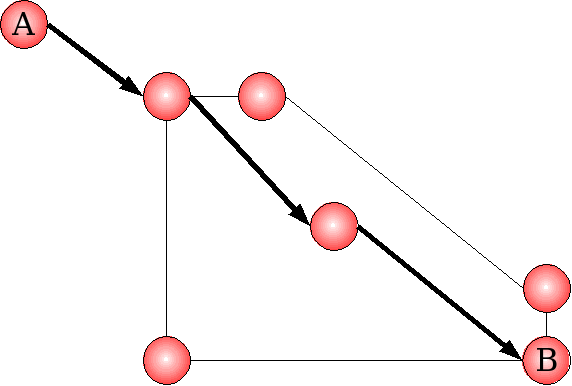
\includegraphics[scale=0.6]{gs1.png}
\caption{"Greedy-Search" in Aktion}
\end{figure}


Leider hat der Algorithmus ein paar Nachteile:

Der Algorithmus ist anfaellig gegenueber falschen Starts:\\
\begin{figure}
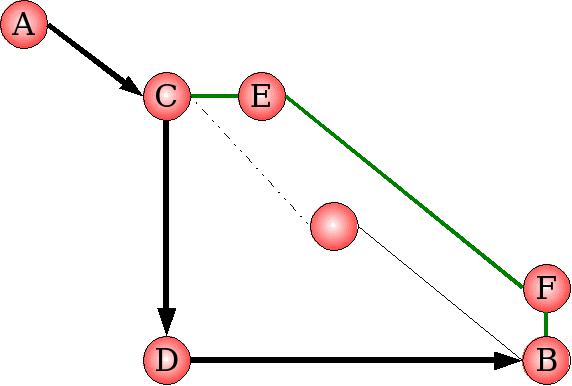
\includegraphics[scale=0.6]{gs2.png}
\caption{"Greedy-Search" ist anfaellig gegenueber falschen Starts}
\end{figure}
                                                                                                                                                            
Und Sackgassen.\\

\begin{figure}
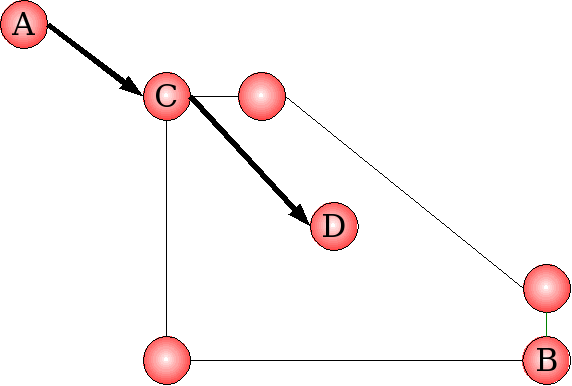
\includegraphics[scale=0.6]{gs3.png}
\caption{"Greedy-Search" ist anfaellig gegenueber Sackgassen}
\end{figure}
                                                                                                                                                            
Oder sogar Schleifen.\\
\begin{figure}
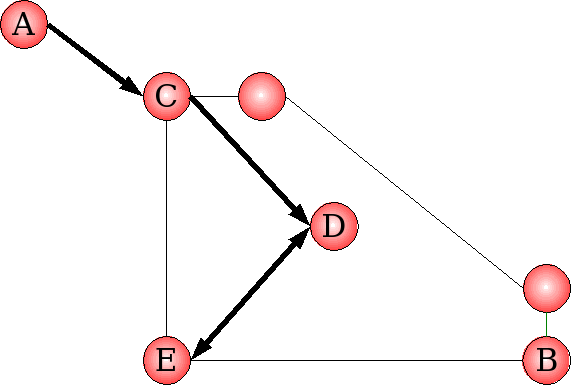
\includegraphics[scale=0.6]{gs4.png}
\caption{"Greedy-Search" ist anfaellig gegenueber Schleifen}
\end{figure}

Greedy Search hat einen Zeitaufwand von O(\(b^{m}\)) im schlechtesten Fall, fuehrt jedoch in vielen Faellen zu einem guten und schnellen Ergebnis.
Wie soeben gesehen ist der GREEDY SEARCH Algorithmus jedoch nicht optimal. Er ist auch nicht vollstaendig, wenn man nicht auf Sackgassen und Schleifen prueft, wie im ersten Teil gezeigt. Leider steigt dann der Speicheraufwand von O(m) auf O(\(b^{m}\)).~~ [7]


\subsection{Verbesserungen von GREEDY SEARCH: A*}

Erweitert man die Funktion i, dass nicht nur die Kinder des gerade geoeffneten sondern aller der noch nicht besuchten Knoten betrachtet ~~~ erhalten wir einen vollstaendigen Algorithmus
Dadurch treten nun keine Schleifen und Sackgassen mehr auf, es wird einfach an die naechste passende Stelle gesprungen.
~~~ Gedaechtnis rausnehmen also naja...

\begin{samepage}
\begin{verbatim}
A* Suche(Zustand alterZustand)
Solange erstelleNeuenZustand(alterZustand,Bewertung) nicht NULL
        Zustand neuerZustand = erstelleNeuenZustand(alterZustand,Bewertung)
liefere als Ergebnis (alterZustand)
                                                                                
Zustand erstelleNeuenZustand(Zustand momentanerZustand,Bewertungsfunktion)
{
        Knoten n = min(Bewertungsfunktion(geoeffnete Knoten von momentaner Zustand))
        Falls oeffneKnoten(momentanerZustand,n) ungleich momentanerZustand
        liefere als Ergebnis oeffneKnoten(momentanerZustand,n)
}
\end{verbatim}
\end{samepage}

\begin{figure}
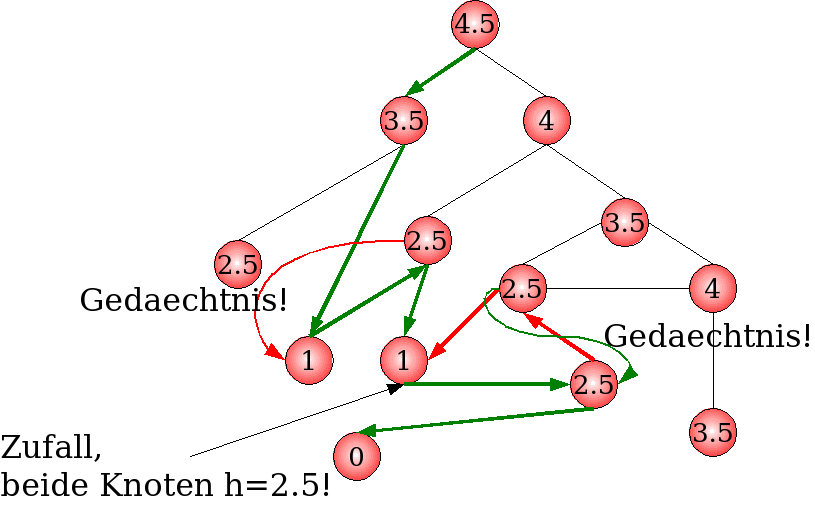
\includegraphics[scale=0.6]{a1.png}
\caption{"Greedy-Search" mit Gedaechtnis}
\end{figure}
                                                                                                                                                            
Leider ist dieser Algorithmus immer noch anfaellig gegenueber einem unguenstigen Start und in vielen Faellen nicht optimal.
Deshalb hat man den sogenannten A* Algorithmus entwickelt, der die gleiche i Funktion aufweist, dessen Bewertungsfunktion h aber eine Kombination aus den bereits bekannten greedy searchs und uniform-cost searchs ist.

Hier ist also h(n) = Enternung von n zum Ziel (Luftlinie) + Kantenlaenge von Start bis n

Bemerkung:
Man kann h auch beliebig anders waehlen, A* bleibt aber nur solange optimal wie die Heuristik h der Dreiecksgleichung genuegt, d.h. zu einer gegebenen Heuristik h und einer direkten Verbindung zweier Punkte A und B darf es keine andere Verbindung zwischen A und B mit einem Knoten C geben, bei der h(B ueber C)<h(B ueber A) gilt. Eine genauere Beschreibung und eine Moeglichkeit derartige heuristische Funktionen zu korrigieren findet man in der Literatur [~~~~].

<BILD mit Dreiecksgleichung>

~~~Untersuchungen erbrachten die Ergebnisse, dass A* optimal und vollstaendig ist und auch, dass es keinen anderen optimalen und vollstaendigen Algorithmus gibt, der (fuer eine beliebige heuristische Funktion) die Aufgabe mit Expandierung von weniger Knoten schafft. [?wo denn~~]

Im Folgenden wird nun anhand des bekannten Beispiels die Funktionsweise von A* demonstriert. Zahlen in den roten Knoten bedeuten wie vorher auch die Distanz mittels Luftlinie, in den gruenen Knoten der Wert der heuristischen Funktion, bisherige Kantenlaenge + Distanz Luftlinie. Ein * markiert einen Knoten, fuer den ein besserer Weg gefunden wurde.
\\
\begin{figure}
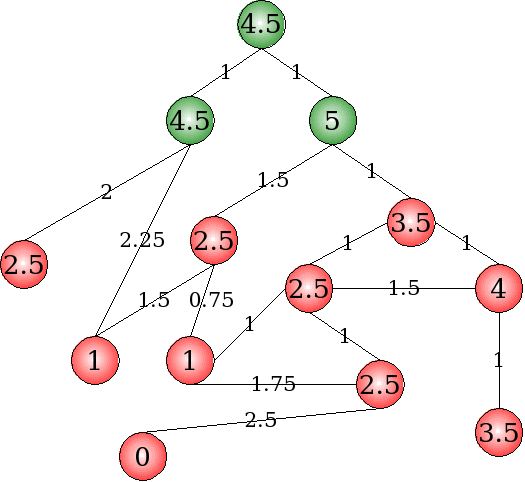
\includegraphics[scale=0.6]{a4.png}
\caption{"A* Search"}
\end{figure}
                                                                                                                                                            
\begin{figure}
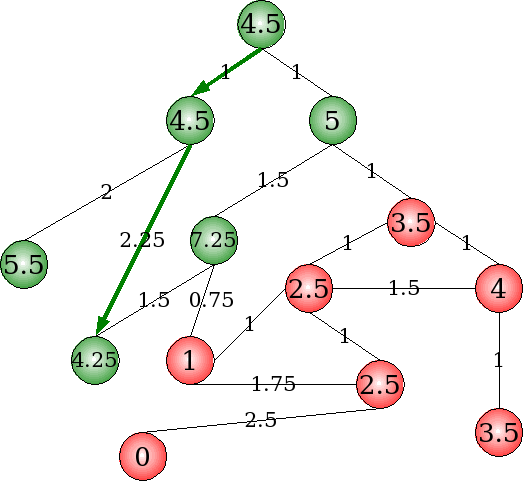
\includegraphics[scale=0.6]{a5.png}
\caption{"A* Search"}
\end{figure}
                                                                                                                                                            
\begin{figure}
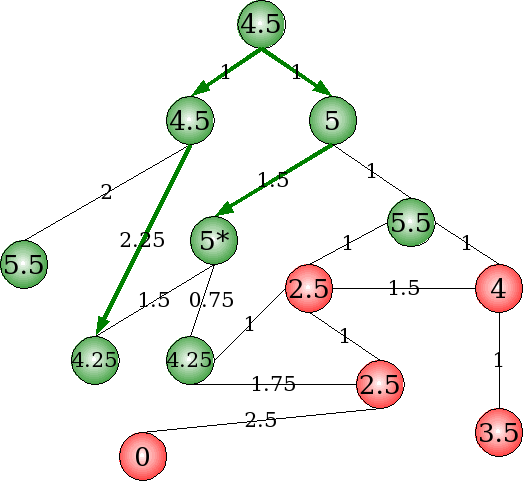
\includegraphics[scale=0.6]{a6.png}
\caption{"A* Search"}
\end{figure}
                                                                                                                                                            
\begin{figure}
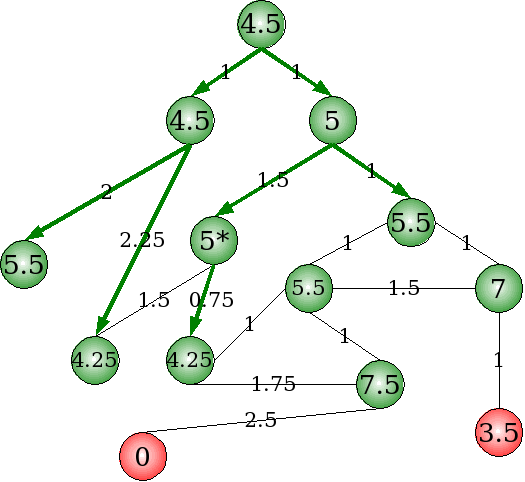
\includegraphics[scale=0.6]{a7.png}
\caption{"A* Search"}
\end{figure}
                                                                                                                                                            
\begin{figure}
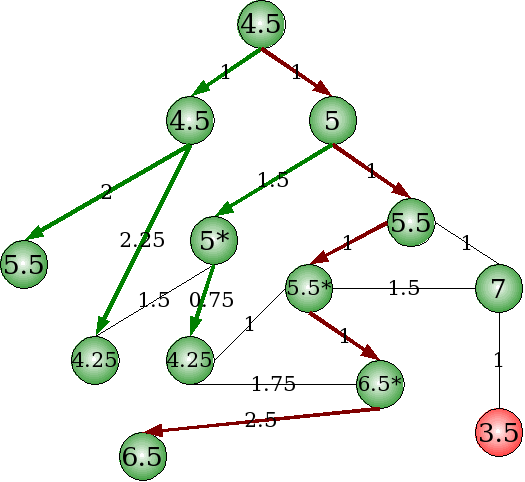
\includegraphics[scale=0.6]{a8.png}
\caption{"A* Search"}
\end{figure}
%~~ Bildbeschreibung                                                                                                                                                            
A* hat in seiner Grundform ebenfalls einen Zeit und Speicheraufwand von O(\(b^{m}\)), da wie beim uniform cost search alle geoeffneten Knoten im Speicher liegen und im schlechtesten Fall auch alle Knoten untersucht werden muessen. 
Fuer b = 2 und m = 40 benoetigt ein Aldi-Rechner fuer A* im schlechtesten Fall vielleicht eine Stunde. Der Speicherbedarf dagegen ist im schlechtesten Fall dagegen mit 1024 GB jenseits von gut und boese.
%Ein verfeinerter Algorithmus der den Speicherverbrauch senkt, waere also nuetzlich. <- das eher im Vortrag
Der Speicheraufwand laesst sich jedoch mit einem etwas abgewandelten Algorithmus reduzieren.

Zum Glueck gibt es derart viele verschiedene, hier werde ich zwei vorstellen:

\subsection{IDA*}

IDA* funktioniert im Grunde wie der bereits betrachtete iterative deepening search, statt Knotentiefe als Grenze wird hier aber ein Kostenlimit gesetzt.
Es werden also immer nur ein Bereich aus Knoten untersucht, deren Bewertungsfunktion h kleiner als das Kostenlimit ist.
Der Speicherersparnis kommt natuerlich fuer den Preis der Geschwindigkeit. Zwar wird nur
IDA* funktioniert genau wie A* auch, es wird aber in mehreren Schritten jeweils immer nur ein Teil des Graphen betrachtet, und zwar der Teil, dessen Knoten eine geringere Qualitaet f~~ besitzen, als ein vorgegebener Wert, der immer weiter erhoeht wird, bis das Ziel gefunden wurde.
~~~~~
\subsection{SMA}

SMA verbraucht keine feste Speichermengenge, sondern passt sich an den verfuegbaren Speicherplatz an, versucht also so viele Knoten wie moeglich zu speichern.
IMA arbeitet genauso wie A* wenn beliebig viel Speicherplatz zur Verfuegung steht.
~~~

\subsection{CSP}

%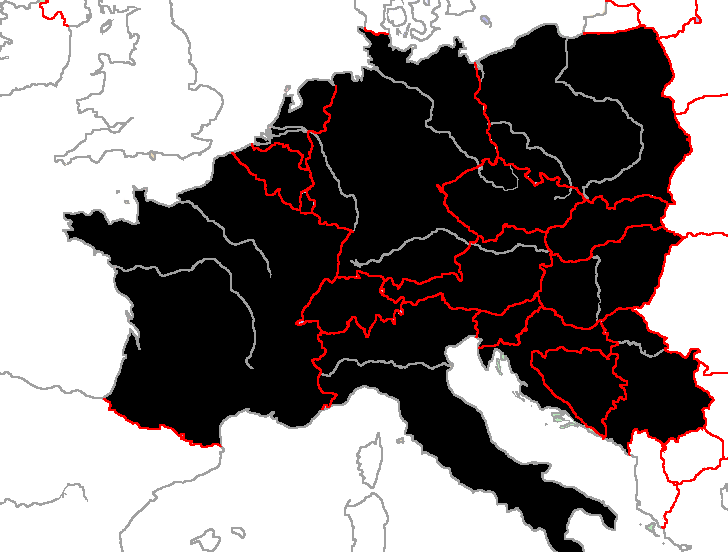
\includegraphics[scale=0.6]{eur11.png}
%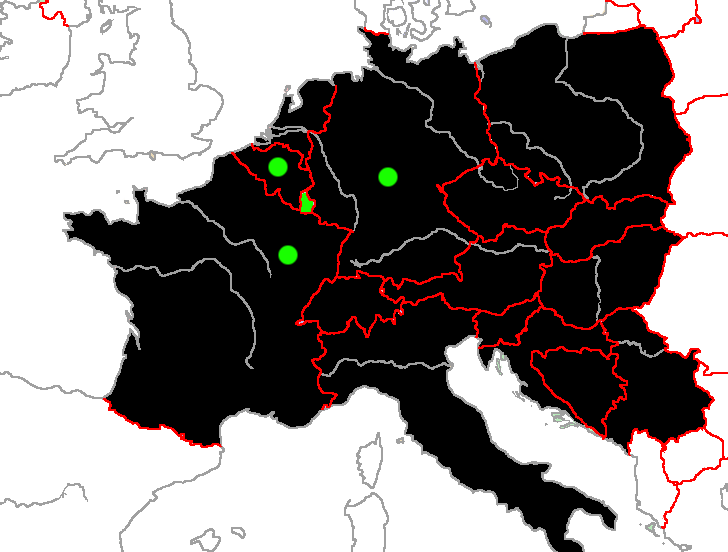
\includegraphics[scale=0.6]{eur12.png}
%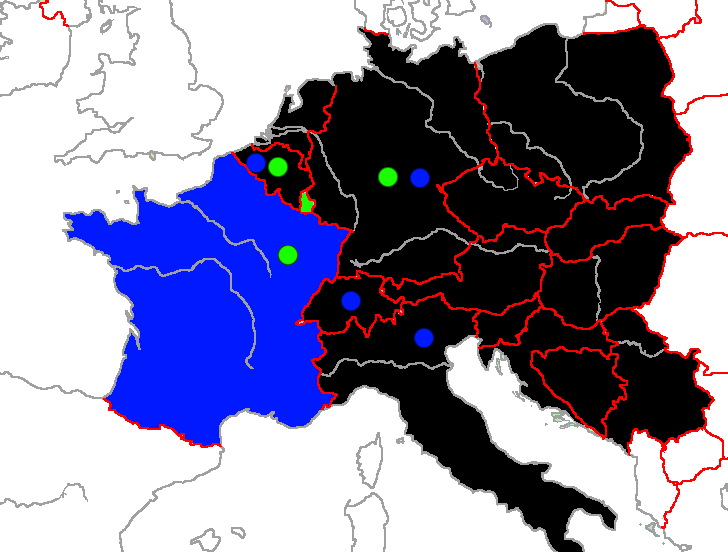
\includegraphics[scale=0.6]{eur13.png}
%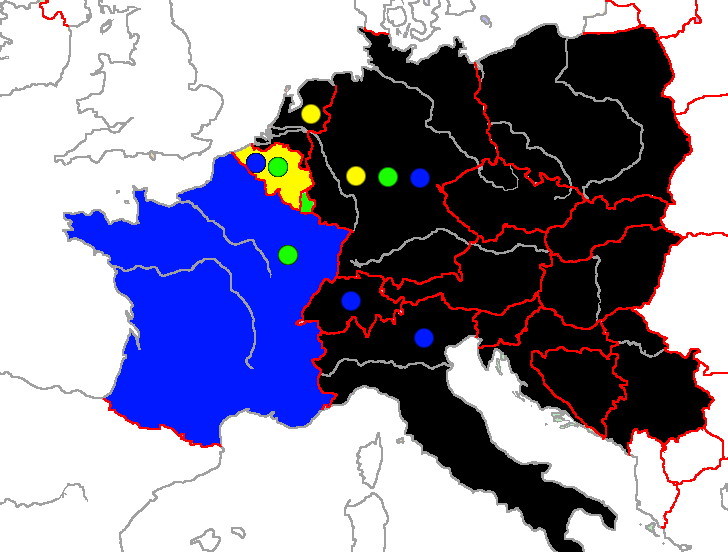
\includegraphics[scale=0.6]{eur14.png}
%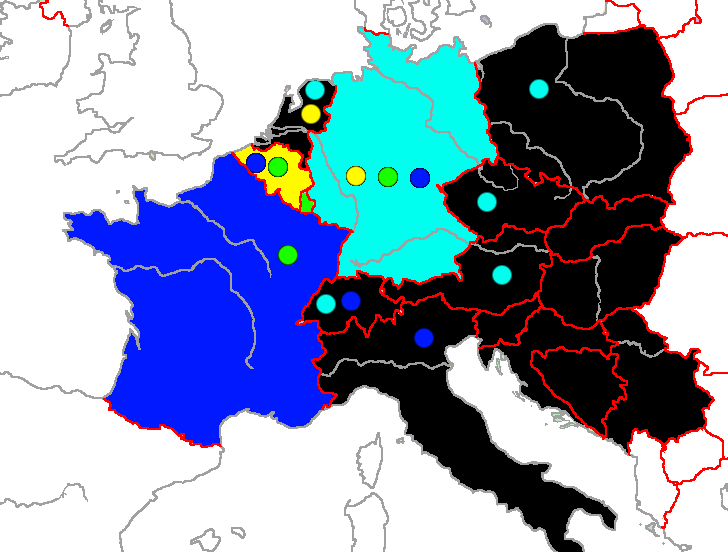
\includegraphics[scale=0.6]{eur15.png}
%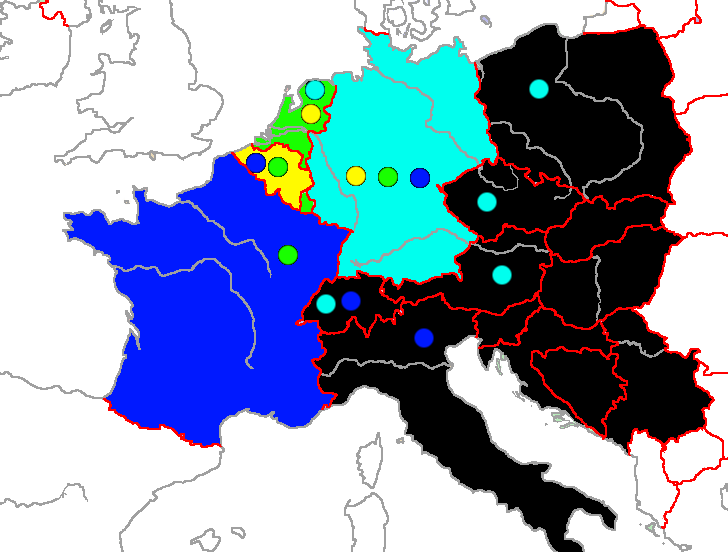
\includegraphics[scale=0.6]{eur16.png}
%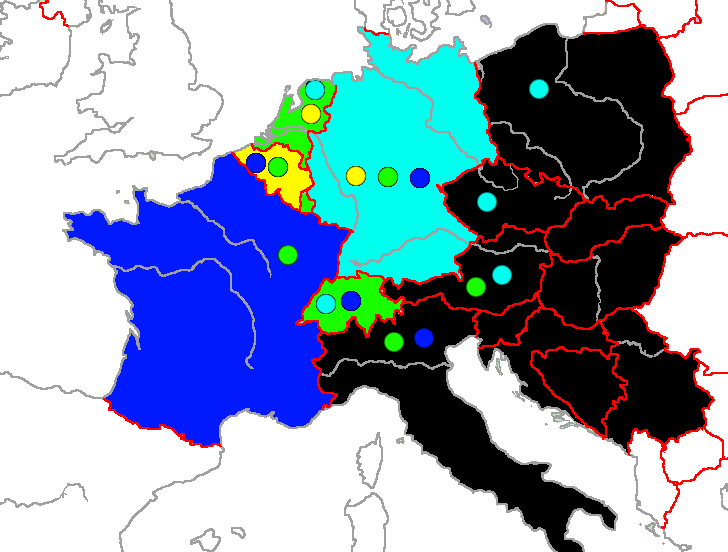
\includegraphics[scale=0.6]{eur17.png}
%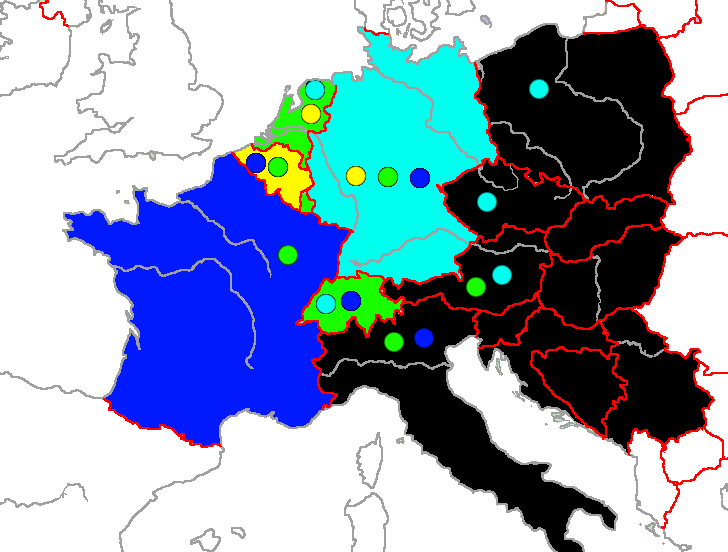
\includegraphics[scale=0.6]{eur18.png}
%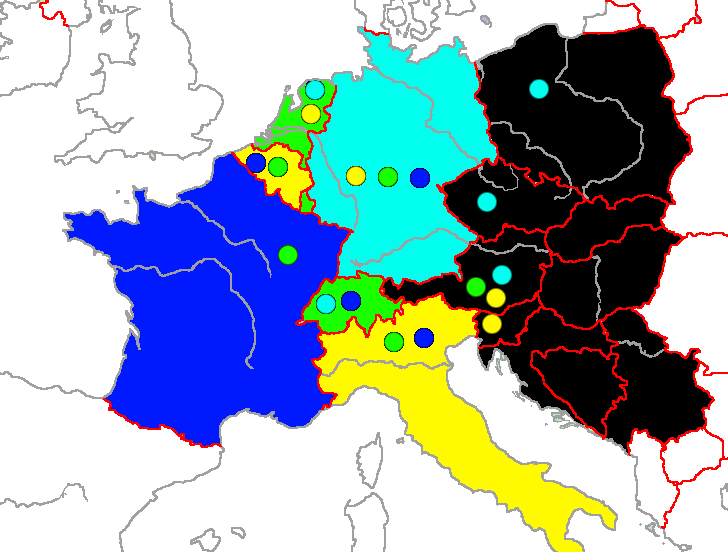
\includegraphics[scale=0.6]{eur19.png}
%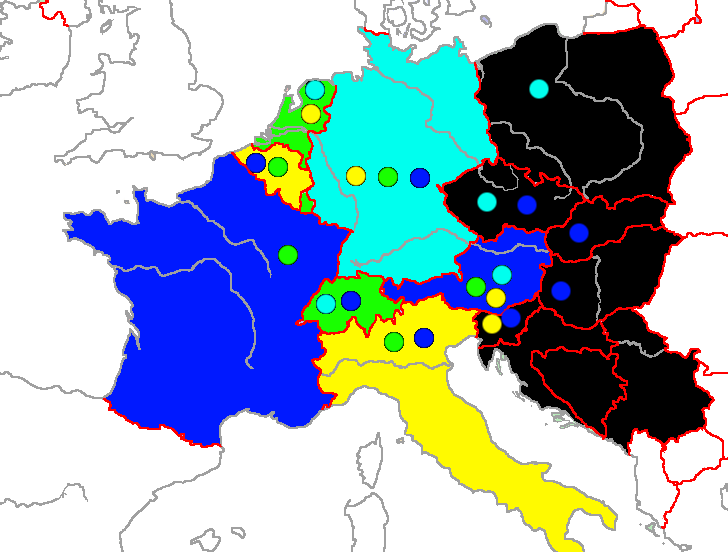
\includegraphics[scale=0.6]{eur20.png}
%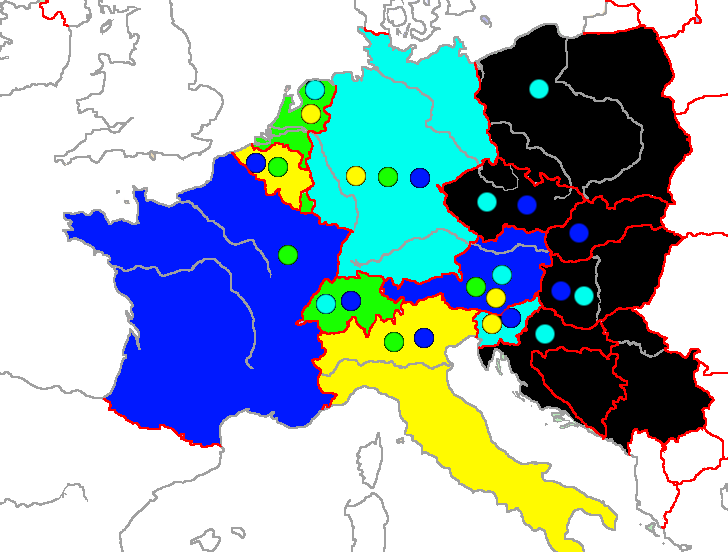
\includegraphics[scale=0.6]{eur21.png}
%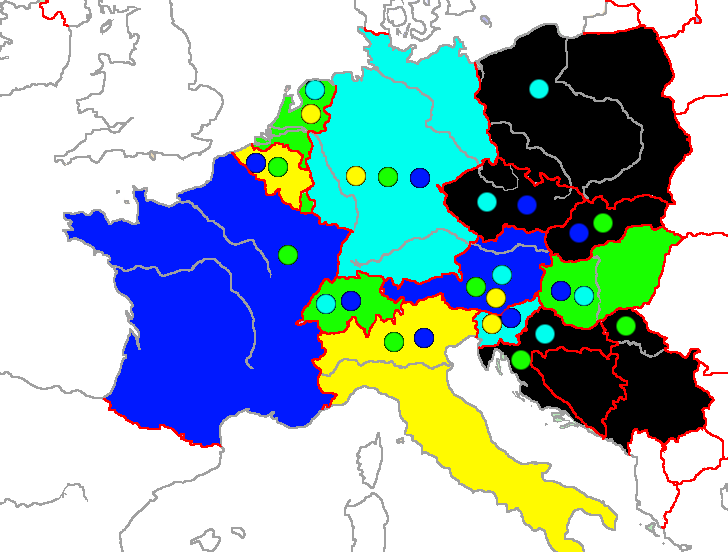
\includegraphics[scale=0.6]{eur22.png}
%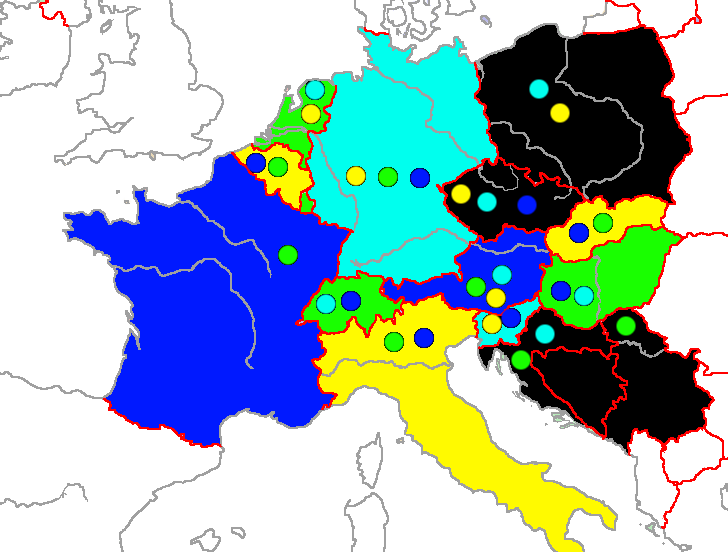
\includegraphics[scale=0.6]{eur23.png}
%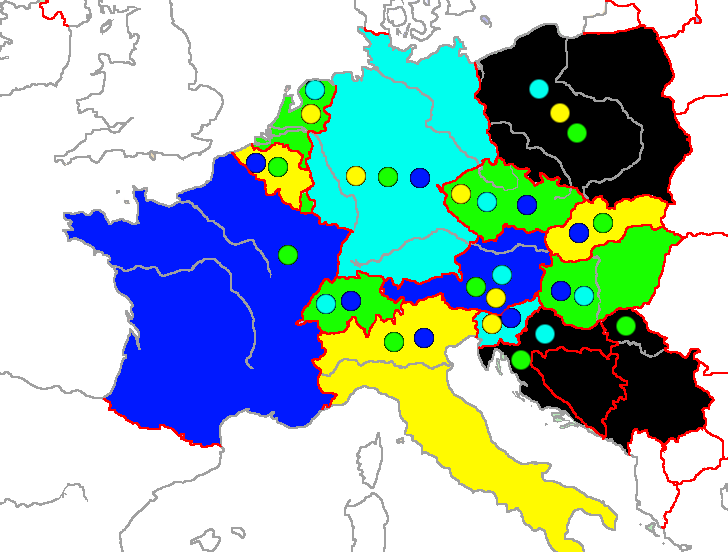
\includegraphics[scale=0.6]{eur24.png}
%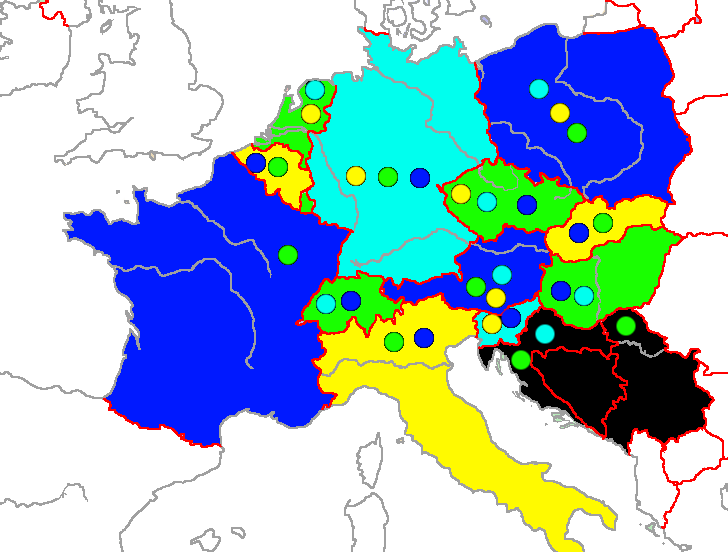
\includegraphics[scale=0.6]{eur25.png}
%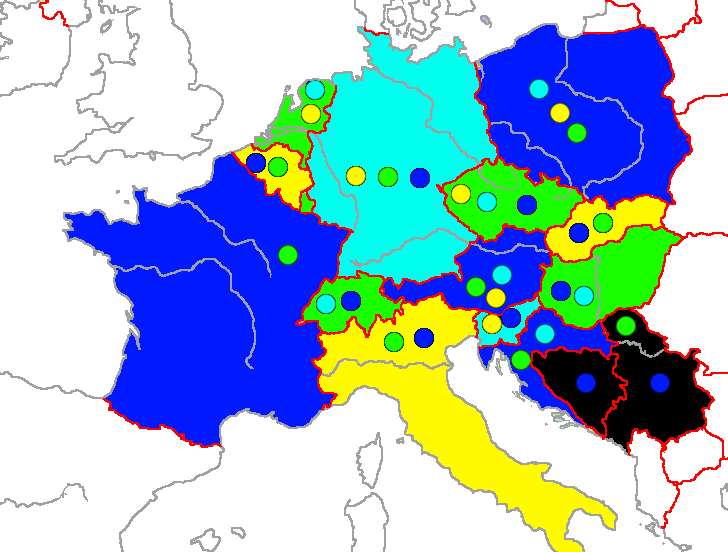
\includegraphics[scale=0.6]{eur26.png}
%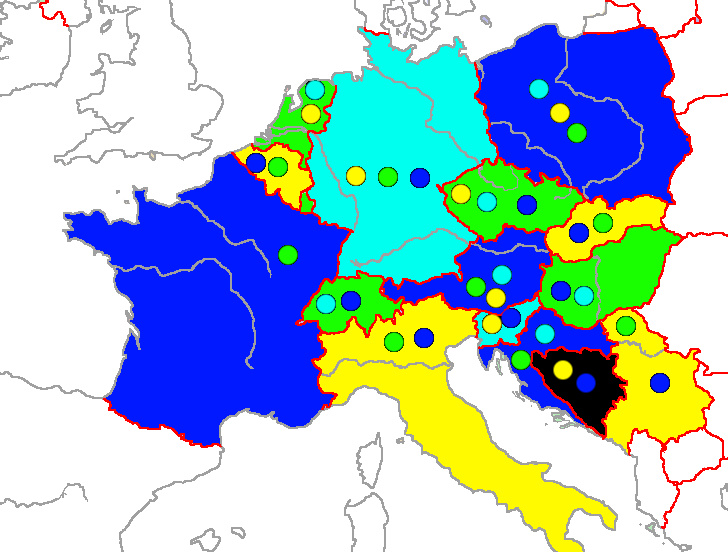
\includegraphics[scale=0.6]{eur27.png}
%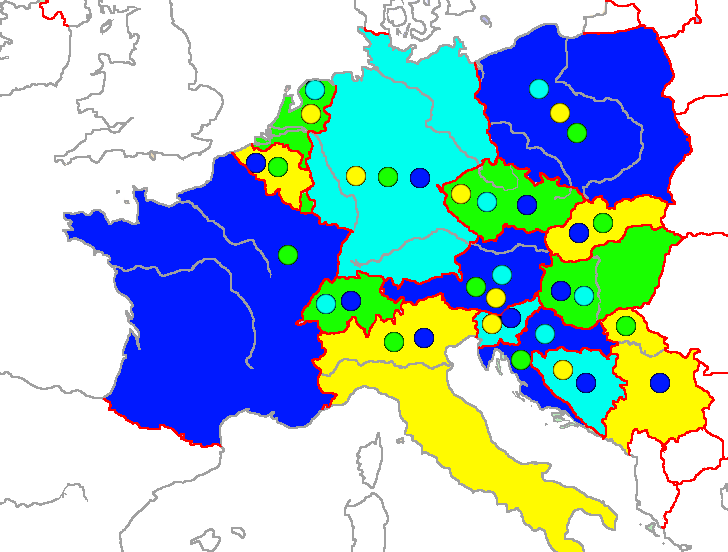
\includegraphics[scale=0.6]{eur28.png}


\section{Algorithmen der 2. Gruppe}

Optimal und vollstaendige Algorithmen sind schoen und gut, in der Praxis sind die Probleme jedoch meist zu komplex oder es liegen sowieso keine gesicherten Werte vor, so dass es oft schon reicht, wenn nicht die optimale Loesung sondern nur z.B. eine 5\% am Optimum liegende Loesung gefunden werden kann.
Diese Aufgabe koennen die Algorithmen der zweiten Gruppe sehr erfolgreich loesen. Wie anfangs erwaehnt werden bei diesen Algorithmen die Loesung nicht Schritt fuer Schritt aufgebaut sondern fertige Loesungen generiert und diese iterativ verbessert.
Wichtig ist dabei, dass die Aufgabenstellung so umgeschrieben wird, dass jede Art von Ergebnis gueltig ist, also einer bestimmten Qualitaetsstufe, der sogenannten Fitness, zugeordnet werden kann.
Dazu werden harte Nebenbedingungen, also z.B. Lagerueberschreitungen, Bargeldueberschreitungen, Zeitueberschreitungen etc. mit Strafkosten belegt, also die Fitness gesenkt, anstatt dass die Loesung ganz verworfen wird.
Der grosse Unterschied zur ersten Gruppe ist aber, dass die neuen Loesungen mehr oder weniger zufaellig generiert werden. Dadurch ergibt sich das Problem, dass man nie genau weiss, ob bei weiteren Durchlaeufen bessere Loesungen gewonnen werden koennen oder nicht.

Grundsaetzlich arbeiten Algorithmen der 2. Gruppe wie folgt:
%~~ englisch/deutscher Name
\begin{samepage}
\begin{verbatim}
basic iterative improvement algorithm()
Loesung alteLoesung = erstelleZufaelligeLoesung()
Wiederhole
        Loesung neueLoesung = i( alteLoesung )
        Differenz = h( neueLoesung) - h( alteLoesung )
	Falls selektion( T, Differenz ) == true
                Dann alteLoesung = neueLoesung
bis alteLoesung ausreichend gut
liefere als Ergebnis alteLoesung
\end{verbatim}
\end{samepage}
%datentyp von Differenz?

Hier sind 2 neue Funktionen hinzugekommen, die jedoch nicht weiter kompliziert sind.
"erstelleZufaelligeLoesung" erstellt wie der Name schon sagt, eine zufaellige Startloesung, die dann schrittweise verbessert werden soll.
"selektion" prueft in Abhaengigkeit einer Variablen T, ob "Differenz" ausreichend klein ist.
Auf einige Beispiele fuer h, i und selektion moechte ich hier eingehen:

\subsection{Hill-Climbing Algorithmus}

Der einfachste darauf basierende Algorithmus ist der sogenannte Hill-Climbing Algorithmus. Der Name ruehrt von dem anschaulichen Problembeispiel her, dass man sich alleine im Gebirge befindet, im Nebel nichts sehen kann, aufgrund Sauerstoffknappheit sich nicht an seine letzten Schritte erinnern kann und als Ziel hat, den hoechsten Berggipfel zu erreichen.
Eine moegliche Strategie waere, dass man sich vortastet, ob man denn mit dem naechsten Schritt etwas hoeher kommt oder nicht.\\

\begin{figure}
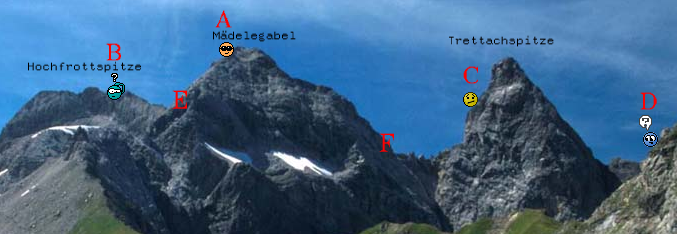
\includegraphics[scale=0.7]{berg.png}
\caption{3 Bergsteiger auf der Suche nach dem Gipfel}
\end{figure} 

\subsection{Probleme des Hill-Climbing Algorithmus}

Bei dem Algorithmus ergeben sich aber zwei schwerwiegende Probleme:

1. der Algorithmus wird mit hoher Wahrscheinlichkeit an einem lokalen Optimum haengenbleiben

Dies laesst sich beheben, indem man den Algorithmus nach einiger Zeit ohne Verbesserung einfach mit einer anderen Startkonfiguration/position neu beginnt, die beste Fitness der bisherigen Durchlaeufe aber speichert. Dann nennt man es einen Random-Restart Hillclimbing Algorithmus. Problem bleibt hier festzustellen, ob wir denn in einem lokalen Optimum oder einer Kante stecken oder nicht schon kurz vor dem Ziel sind.

<BILD20!>

2. ist die Fitnesslandschaft sehr "wild" also mit grossen Gradientenunterschieden besetzt

Hier hilft auch kein zufaelliges Neustarten mehr, man wird wahrscheinlich fast alle Loesungsmoeglichkeiten durchsuchen muessen, der Algorithmus ist also nicht viel besser als eine einfache zufaellige Suche ueber dem Loesungsraum.
Die Hauptschwierigkeit beim Hillclimber ist also nicht die Suche selbst sondern die Gestaltung der Problemstellung, so dass eine Fitnesslandschaft mit moeglichst sanften Steigungen entsteht.

<BILD22!>

/*Eine weitere Variante des Hillclimbers waere, anstatt die absoluten Werte der Loesungen zu vergleichen, die Gradienten herzunehmen.
Bei praktischen Problemen mit hunderten von Variablen erweist sich dies aber als nicht praktikabel, da man hierzu die Ableitung der Fitnessfunktion bestimmen muesste.
Und wer will schon eine Funktion mit Schleifen, Zufallswerten, Rekursionen und Spruengen differenzieren... :-)
*/

\subsection{Simulated Annealing Algorithmus}

Aehnlich funktioniert auch das sogenannte Simulated Annealing, das urspruenglich aus der Physik kommt.
Wird eine bessere Loesung gefunden, wird sie wie beim Hillclimber auf jeden Fall weiterverwendet, wird eine schlechtere Loesung gefunden, wird sie nicht sofort verworfen, sondern mit einer Wahrscheinlichkeit die der Parameter T angibt weiterverwendet.
Ueber die Generationen wird T dabei immer weiter verringert, bis fuer T=0 (hoffentlich) eine ziemlich gute Loesung gefunden wurde.

<BILD, Beispiel Transportstrecke zwischen Staedte>

O------------O
|            |
|            |
|            |
|            |
o------------o


\subsection{Anwendungen in CSPs : Heuristik des minimalen Konflikts~~}

Heuristische Algorithmen der 2. Gruppe eignen sich sehr gut, um CSP Probleme wie z.B. das n-Damenproblem zu loesen. Mit der nun beschriebenen Heuristik kann z.B. das Millionen-Damen Problem im Durschnitt mit weniger als 50 Schritten geloest werden. [5]

Wieder ist der Trick, nicht perfekte Loesungen zu suchen, sondern eine zufaellige zu generieren diese Schritt fuer Schritt zu "reparieren" (~~ heuristic repair).
Das Optimierungsproblem zu n-Dameproblem lautet "Finde eine Position in der moeglichst wenige Damen von moeglichst wenigen anderen Damen geschlagen werden koennen".                                                                  

Hier nun zur Uebersicht ein Beispiel zum 4 Dameproblem in 5 Schritten:

Waehrend die roten Felder die Positionen der 4 Damen darstellen, geben die Zahlen den Wert der Heuristik an.
Die Heuristik ist eine sogenannte "min conflicts"[6] Heuristik, die jeweils angibt, wieviele Bedingungen bei einer Konfiguration ueberschritten wird.
In diesem Fall entspricht dies der Zahl der Damen, die das Feld angreifen, bei roten Feldern inklusive dieser Dame selbst.
Bei jedem Reperaturschritt der ungueltigen Loesung wird nun fuer eine Dame einer zufaelligen Spalte ein zufaellig Feld mit niedrigerer oder gleicher Bewertung gewaehlt.

%Programm evtl?

\begin{figure}
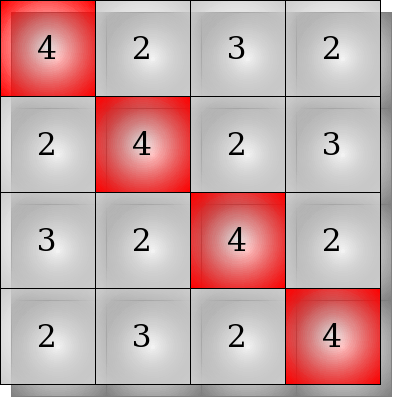
\includegraphics[scale=0.6]{dame1.png}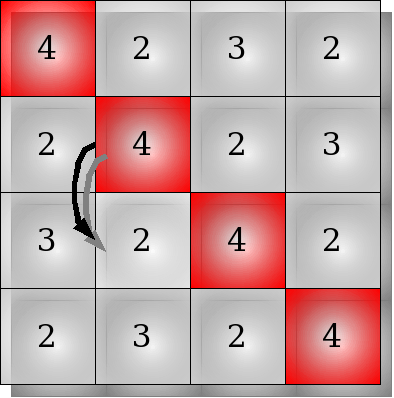
\includegraphics[scale=0.6]{dame2.png}
\caption{"CSP" mittels Heuristik des minimalen Konflikts}
\end{figure}
                                                                                                                                                            
In diesem Beispiel stehen alle 4 Damen in einer Diagonalen, also koennen z.B. in der Diagonalen 4 Damen jeweils ein Feld angreifen bzw. stehen darauf~~. 
Hier wurde die 2. Spalte gewaehlt und die Dame auf das niedriegere Feld in der 3. Zeile verschoben.
Dass diese Heuristik scheinbar funktioniert, kann man auch daran erkennen, dass die Gesamtzahl der angegriffenen Damen sich von 16 nun auf 8 verringert hat:

\begin{figure}
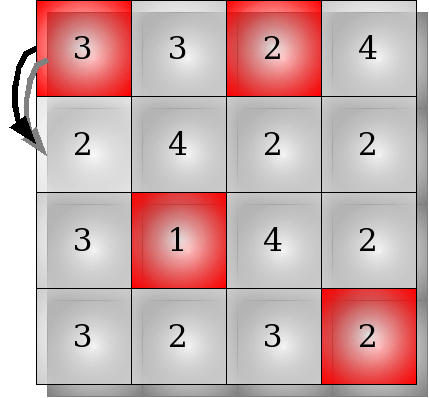
\includegraphics[scale=0.6]{dame3.png}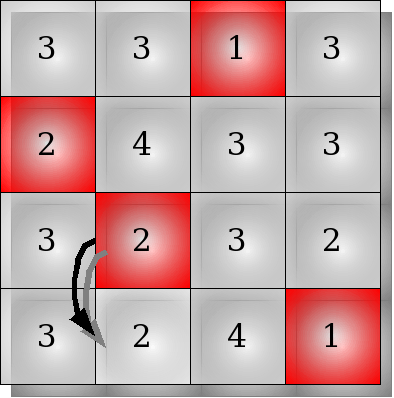
\includegraphics[scale=0.6]{dame4.png}
\caption{"CSP" mittels Heuristik des minimalen Konflikts}
\end{figure}
                                                                                                                                                            
Im ersten Bild ist hier die Wahl der ersten Spalte zwingend, mit keiner anderen Dame findet man ein besseres Feld.
In der Situation im zweiten Bild wuerde der Hill-Climber sich auf einem Plateau befinden und waere nicht besser wie eine zufaellige Suche. Man koennte hier anstatt nur die einzelnen Felder im Ursprungszustand betrachten, die Gesamtzahl der sich ueberschneidenden Damen eintragen, was aber mit einem Aufwand von O(n Damen*n*n Felder) verbunden waere~~. Beweis?~~

\begin{figure}
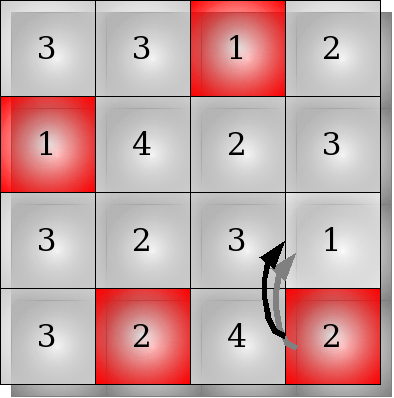
\includegraphics[scale=0.6]{dame5.png}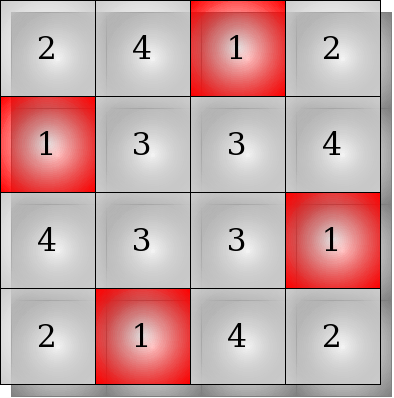
\includegraphics[scale=0.6]{dame6.png}
\caption{"CSP" mittels Heuristik des minimalen Konflikts}
\end{figure}
                                                                                                                                                            
Im letzten Bild gibt es keine Verbesserung und der Hill-Climber laeuft ohne Verbesserung bis zum Abbruch ohne Veraenderung weiter. Da wir aber das Optimum, d.h. es gibt eine Loesung fuer das n-Damenproblem mit keiner Ueberschneidung, schon kennen und es hier auch abzaehlen koennen, sind wir fertig.

\subsection{Verfeinerung des Hill-Climbing Algorithmus}

Es gibt einige Verfeinerungen des Hill-climbing Algorithmus, besonders erwaehnenswert sind Genetische Algorithmen/Programmierung und Evolutionaere Algorithmen.

Diese finden z.B. Anwendung in komplexen praktischen Problemstellungen wie z.B. Betriebsplanoptimierung an der schon laenger SAP erfolgreich arbeitet.

BAECKER!!

neurale netzwerke
Algorithmen der zweiten Gruppe sind, sofern man nicht den Weg ueber neurale Netzwerke begeht, nur bei bestimmten Problemen einsetzbar. Schachspielen ist z.B. nicht moeglich, da dort ja nicht nur ein Spielablauf optimiert werden soll, sondern moeglichst jede Antwort auf jeden Zug ~~`

~~~ Grob gesagt handelt es sich bei GAs um Hillclimber mit einer Breitensuche in Form von einer Population von "Agenten", mit einer Trennung von Genotyp, also der tatsaechlichen Genstruktur und Phaenotyp, also dem entgueltigen Erscheinungsbild, mit einer Art Gedaechtnis in Form von dominant/rezessiver Gene und inaktiver Gene, sogenannter Introne, die nicht tatsaechlich in einen Phaenotyp codiert werden, sondern nur als Mutationsschutz dienen und mit einer Rekombination durch Crossing Over zwischen den Agenten.

Genauer kann ich leider nicht darauf eingehen, das wuerde den Rahmen des Vortrags sprengen, wer sich damit etwas beschaefitgen will, dem empfehle ich das Buch "Genetic Programming - An introduction".
Sie sind sehr erfolgreich, verglichen mit anderen Suchstrategien, denn welch anderer Algorithmus kann schon Vortraege ueber sich selbst halten?

----------


Bevor man sich ueberhaupt Gedanken machen kann, welchen Suchalgorithmus man auf ein spezielles Problem anwendet, ist es unabdingbar, dass man sich ueberlegt, wie man 2 Loesungen vergleicht. Dies stellt die Zielfunktion dar, die entweder maximiert, wie z.B. bei Gewinnspannen oder minimiert, wie z.B. bei Entfernungen werden soll.

Zwar fuehrt das Absuchen des kompletten Loesungsraums wie im 1. Teil besprochen garantiert zur optimalen Loesung, jedoch sind die meisten Probleme einfach zu komplex um sie derartig auszurechnen.
Als Beispiel waere Schach genannt, bei der eine Partie oft um die 40 Zuege dauert. Da der Computer sowohl den optimalen eigenen, als auch den optimalen gegnerischen Zug berechnen muesste, waeren das \(10^{80}\) Stellungen die miteinander verglichen werden muessten.

Bei heuristischen Suchverfahren verlaesst man sich deshalb nicht auf das sichere Ereignis, wie z.B. "Mit diesem Zug gewinne ich die Partie nach 40 Zuegen, sofern der Gegner optimal spielt", sondern mit gewissen Annahmen die fuer jedes Problem einzeln ueberlegt werden muessen.
Um auf das Schachbeispiel zurueckzukommen:
Moderne Schachcomputer rechnen nicht jede Zugkombination bis zum Ende der Partie durch, sondern vergleichen schon nach wenigen Zuegen die Zahl und Position der Figuren um die Stellung bewerten zu koennen und auf ein eindimensionales Ergebnis zu kommen.
Das Wissen um die Qualitaet einer Stellung im Schach wurde aber nicht berechnet sondern mehr oder weniger durch Versuch und Irrtum bestimmt.


Betrachtet man hierbei nicht alle moeglichen 


%In der Zusammenfassung steht nochmals kondensiert der Kerninhalt der Ausarbeitung
%Das, was der Leser danach wissen sollte.
\section{Zusammenfassung}

\subsection{Allgemeine Suchalgorithmen}


\subsection{Heuristische Suchalgorithmen}

Insgesamt hat man im zweiten Teil gesehen, dass wir die Zahl der zu untersuchenden Moeglichkeiten durch Heuristiken stark reduzieren koennen. Zwar bieten die Heuristiken keine Garantie fuer eine schnellere Ausfuehrung, die schlechteste Laufzeit betraegt nach wie vor O(\(b^{m}\)), im praktischen Anwendungsfall mit einer guten Heuristik laesst sich jedoch die durchschnittliche Suchzeit stark reduzieren.

Begonnen haben wir mit einer allgemeinen Beschreibung der heuristischen Funktion, die man sich als eine Art Orakel vorstellen kann das Informationen ausserhalb des Wahrnehmungsbereichs der generalisierten Suche aufnimmt, und die jeweilige Loesung nach ihrer bewertet.

...


\begin{thebibliography}{99}
\bibitem{Norv03} {\sc Russel S., Norvig P.:}  \textit{Artificial Intelligence -- A Modern Approach}, 
Second Edition, Prentice Hall, 2003.
\bibitem{Worldmap} {\sc Brion L. Vibber:}  \textit{Maps of the World},
http://leuksman.com/misc/maps.php
%evtl noch benutzte Software eintragen, openoffice, vim, gimp, texi2pdf
\end{thebibliography}
%TODO: Fett/Kursiv rein, Sonderzeichen etc.
\end{document}

